\section*{Routine Problems:}

It is expected that the following activities will allow you to understand, review, and use analytical methods: integrating factor, separable variables, and exact equations (among others). Furthermore, that the development of these activities generates feelings of confidence in you when solving some first-order ordinary differential equations.

\vspace{1em}

\textbf{Activity 1. Perform exercises 1 through 16 on page 33 of [2], submit 4, 8, 10, 12, 13, 14, and 16.}
\begin{quote}


\noindent In each of Problems 1 through 8:
\begin{enumerate}
    \item Draw a direction field for the given differential equation.
    \item Based on an inspection of the direction field, describe how solutions behave for large $t$.
    \item Find the general solution of the given differential equation, and use it to determine how solutions behave as $t \to \infty$.
\end{enumerate}

\begin{center}
    \rule{0.5\textwidth}{0.5pt}
\end{center}


\textbf{4. $y' + \frac{1}{t}y = 3\cos(2t), \quad t > 0$}
\begin{respuesta}


\textbf{1.}Draw a direction field for the given differential equation.
\begin{figure}[H]
    \centering
    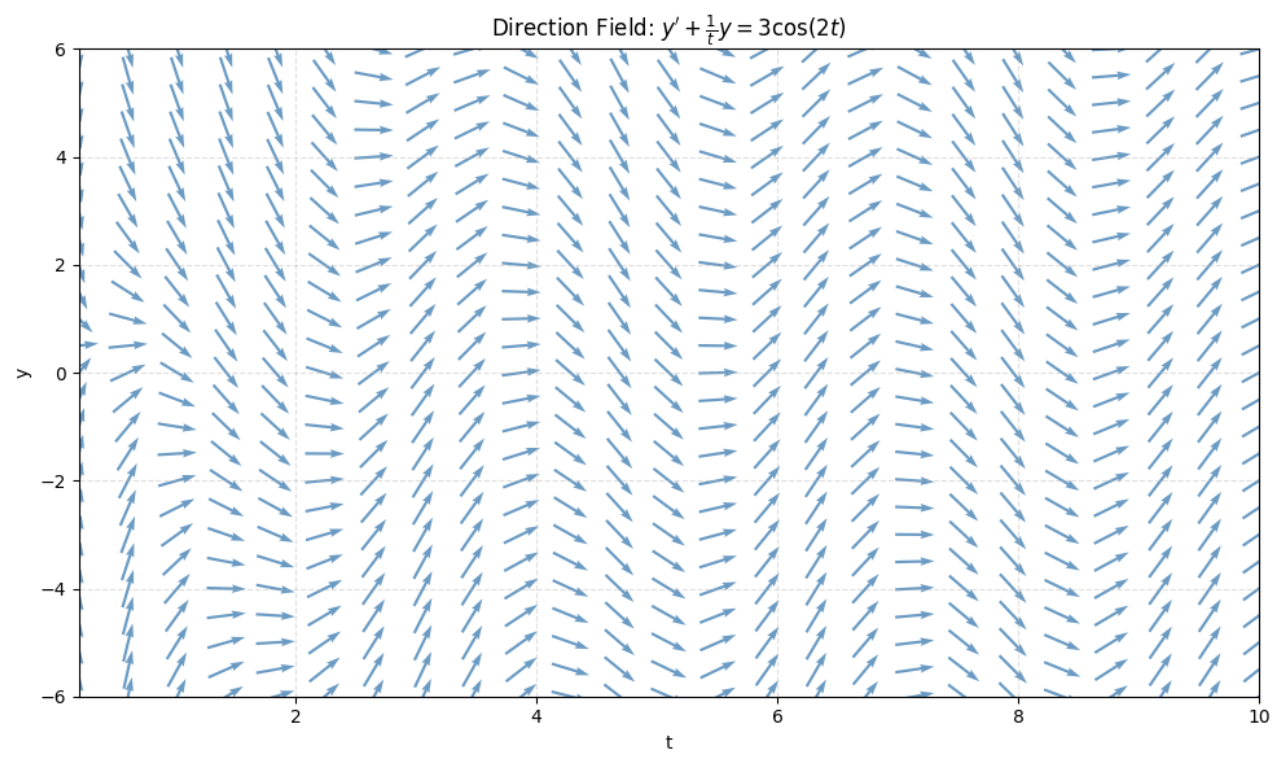
\includegraphics[width=0.8\textwidth]{secciones/michael/images/DF_4.png}
    \caption{Direction field for $y' + \frac{1}{t}y = 3\cos(2t)$}
    \label{fig:dirfield}
\end{figure}

\textbf{2.}Based on an inspection of the direction field, describe how solutions behave for large $t$.

For large $t$, the direction field shows that all solutions appear to oscillate in a wave-like pattern. Regardless of the initial condition, the solutions seem to be attracted toward the same repeating oscillation, suggesting that any transient behavior dies out over time and every solution eventually behaves like a sinusoidal wave of fixed amplitude.


\textbf{3.}Find the general solution of the given differential equation, and use it to determine how solutions behave as $t \to \infty$.

The equation is already in standard form $y' + \frac{1}{t}y = 3\cos(2t)$, so the integrating factor is:
\[
\mu(t) = e^{\int \frac{1}{t}\,dt} = e^{\ln t} = t
\]
Multiplying both sides by $\mu(t) = t$:
\[
ty' + y = 3t\cos(2t) \implies \frac{d}{dt}(ty) = 3t\cos(2t)
\]
Integrating both sides (by parts on the right side, with $u = 3t$, $dv = \cos(2t)\,dt$):
\[
ty = \frac{3t}{2}\sin(2t) + \frac{3}{4}\cos(2t) + C
\]
Dividing by $t$, the general solution is:
\[
y = \frac{3}{2}\sin(2t) + \frac{3}{4t}\cos(2t) + \frac{C}{t}
\]
As $t \to \infty$, the transient terms vanish since $\frac{3}{4t}\cos(2t) \to 0$ and $\frac{C}{t} \to 0$, so all solutions satisfy:
\[
y \to \frac{3}{2}\sin(2t) \quad \text{as } t \to \infty
\]
regardless of the initial condition.


\end{respuesta}


\begin{center}
    \rule{0.5\textwidth}{0.5pt}
\end{center}


\textbf{8. $2y' + y = 3t^2$}
\begin{respuesta}

\textbf{1.}Draw a direction field for the given differential equation.
\begin{figure}[H]
    \centering
    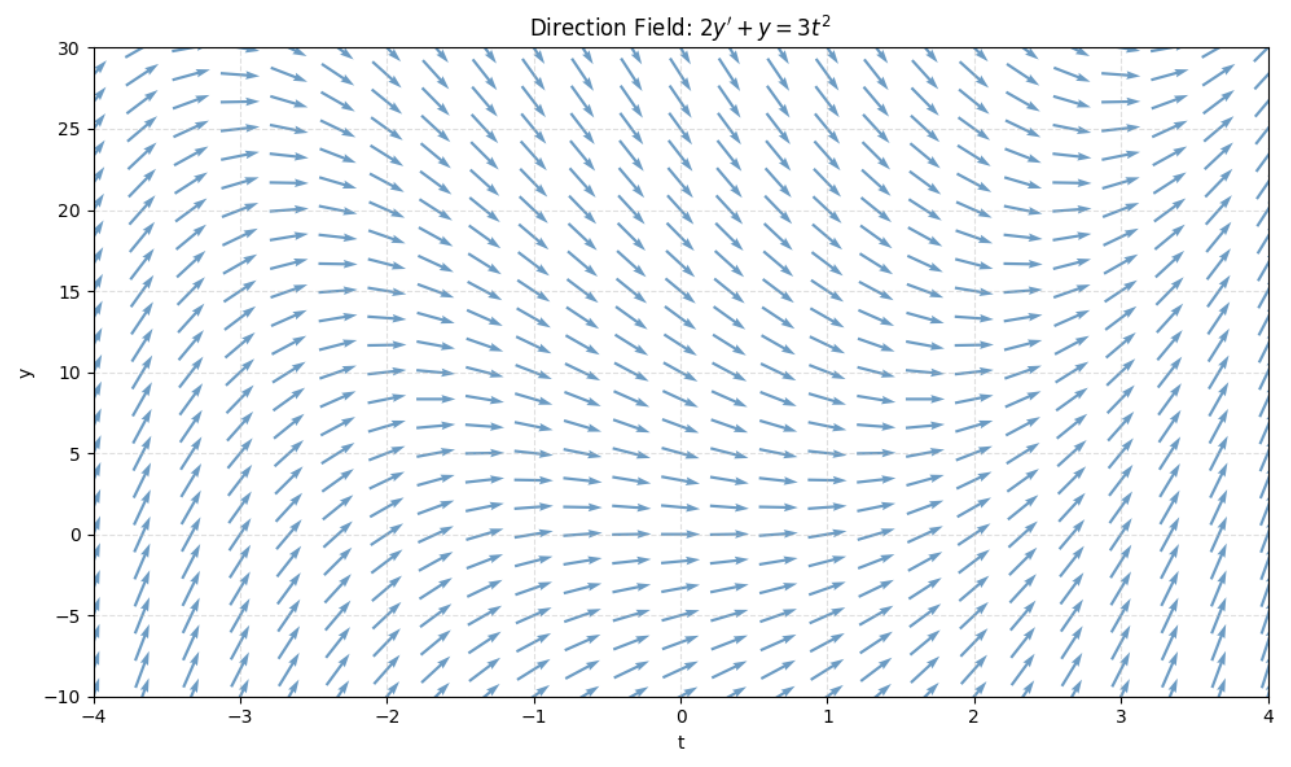
\includegraphics[width=0.8\textwidth]{secciones/michael/images/DF_8.png}
    \caption{Direction field for $2y' + y = 3t^2$}
    \label{fig:dirfield}
\end{figure}

\textbf{2.}Based on an inspection of the direction field, describe how solutions behave for large $t$.

For large $t$, the direction field shows that all solutions grow without bound. The slopes become increasingly steep and positive as $t$ increases, suggesting that every solution diverges to infinity regardless of the initial condition.


\textbf{3.}Find the general solution of the given differential equation, and use it to determine how solutions behave as $t \to \infty$.

Rewriting in standard form by dividing by $2$:
\[
y' + \frac{1}{2}y = \frac{3}{2}t^2
\]
The integrating factor is:
\[
\mu(t) = e^{\int \frac{1}{2}\,dt} = e^{t/2}
\]
Multiplying both sides by $\mu(t) = e^{t/2}$:
\[
\frac{d}{dt}\left(e^{t/2}y\right) = \frac{3}{2}t^2 e^{t/2}
\]
Integrating the right side by parts twice:
\[
e^{t/2}y = 3t^2e^{t/2} - 12te^{t/2} + 24e^{t/2} + C
\]
Dividing by $e^{t/2}$, the general solution is:
\[
y = 3t^2 - 12t + 24 + Ce^{-t/2}
\]
As $t \to \infty$, the transient term $Ce^{-t/2} \to 0$, so all solutions behave like:
\[
y \to 3t^2 - 12t + 24 \quad \text{as } t \to \infty
\]
which grows without bound, confirming that all solutions diverge to $+\infty$ regardless of the initial condition.

\end{respuesta}




% ---------------------------------------------------
\noindent In each of Problems 9 through 12, find the solution of the given initial value problem.
\begin{center}
    \rule{0.5\textwidth}{0.5pt}
\end{center}


\textbf{10.  $y' + 2y = te^{-2t}, \quad y(1) = 0$}
\begin{respuesta}

\textbf{Integrating Factor.} This is a first-order linear ODE of the form
$y' + p(t)y = g(t)$, with $p(t) = 2$. The integrating factor is:
\[
\mu(t) = e^{\int 2\, dt} = e^{2t}
\]

\textbf{Multiplying both sides} by $\mu(t) = e^{2t}$:
\[
e^{2t}y' + 2e^{2t}y = te^{-2t} \cdot e^{2t} = t
\]

The left-hand side is an exact derivative:
\[
\frac{d}{dt}\!\left(e^{2t}y\right) = t
\]

\textbf{Integrating both sides} with respect to $t$:
\[
e^{2t}y = \int t\, dt = \frac{t^2}{2} + C
\]

\textbf{General solution:}
\[
y = \left(\frac{t^2}{2} + C\right)e^{-2t}
\]

\textbf{Applying the initial condition} $y(1) = 0$:
\[
0 = \left(\frac{1}{2} + C\right)e^{-2} \implies \frac{1}{2} + C = 0 \implies C = -\frac{1}{2}
\]

\textbf{Solution:}
\[
\boxed{y = \frac{t^2 - 1}{2}\,e^{-2t}}
\]

\end{respuesta}



\begin{center}
    \rule{0.5\textwidth}{0.5pt}
\end{center}


\textbf{12. $ty' + (t + 1)y = t, \quad y(\ln 2) = 1, \quad t > 0$}
\begin{respuesta}

\textbf{Standard Form.} Divide both sides by $t$ to write the equation in standard linear form:
\[
y' + \frac{t+1}{t}\,y = 1 \quad \Longrightarrow \quad y' + \left(1 + \frac{1}{t}\right)y = 1
\]

\textbf{Integrating Factor.} With $p(t) = 1 + \tfrac{1}{t}$:
\[
\mu(t) = e^{\int\!\left(1 + \frac{1}{t}\right)dt} = e^{t + \ln t} = te^{t}
\]

\textbf{Multiplying both sides} by $\mu(t) = te^{t}$:
\[
te^{t}y' + (t+1)e^{t}y = te^{t}
\]

The left-hand side is an exact derivative:
\[
\frac{d}{dt}\!\left(te^{t}y\right) = te^{t}
\]

\textbf{Integrating both sides} with respect to $t$ (using integration by parts on the right):
\[
te^{t}y = \int te^{t}\,dt = e^{t}(t - 1) + C
\]

\textbf{General solution:}
\[
y = \frac{t-1}{t} + \frac{Ce^{-t}}{t}
\]

\textbf{Applying the initial condition} $y(\ln 2) = 1$:
\[
1 = \frac{\ln 2 - 1}{\ln 2} + \frac{C e^{-\ln 2}}{\ln 2} = \frac{\ln 2 - 1}{\ln 2} + \frac{C}{2\ln 2}
\]
\[
1 - \frac{\ln 2 - 1}{\ln 2} = \frac{C}{2\ln 2} \implies \frac{1}{\ln 2} = \frac{C}{2\ln 2} \implies C = 2
\]

\textbf{Solution:}
\[
\boxed{y = \frac{t - 1 + 2e^{-t}}{t}}
\]

\end{respuesta}


% ---------------------------------------------------

\noindent In each of Problems 13 and 14:

\begin{enumerate}
    \item Draw a direction field for the given differential equation. How do solutions appear to behave as $t$ becomes large? Does the behavior depend on the choice of the initial value $a$? Let $a_0$ be the value of $a$ for which the transition from one type of behavior to another occurs. Estimate the value of $a_0$.
    \item Solve the initial value problem and find the critical value $a_0$ exactly.
    \item Describe the behavior of the solution corresponding to the initial value $a_0$.
\end{enumerate}

\begin{center}
    \rule{0.5\textwidth}{0.5pt}
\end{center}



\textbf{13. $y' - \frac{1}{2}y = 2\cos(t), \quad y(0) = a$}
\begin{respuesta}

\textbf{1. }Draw a direction field for the given differential equation. How do solutions appear to behave as $t$ becomes large? Does the behavior depend on the choice of the initial value $a$? Let $a_0$ be the value of $a$ for which the transition from one type of behavior to another occurs. Estimate the value of $a_0$.
\begin{figure}[H]
    \centering
    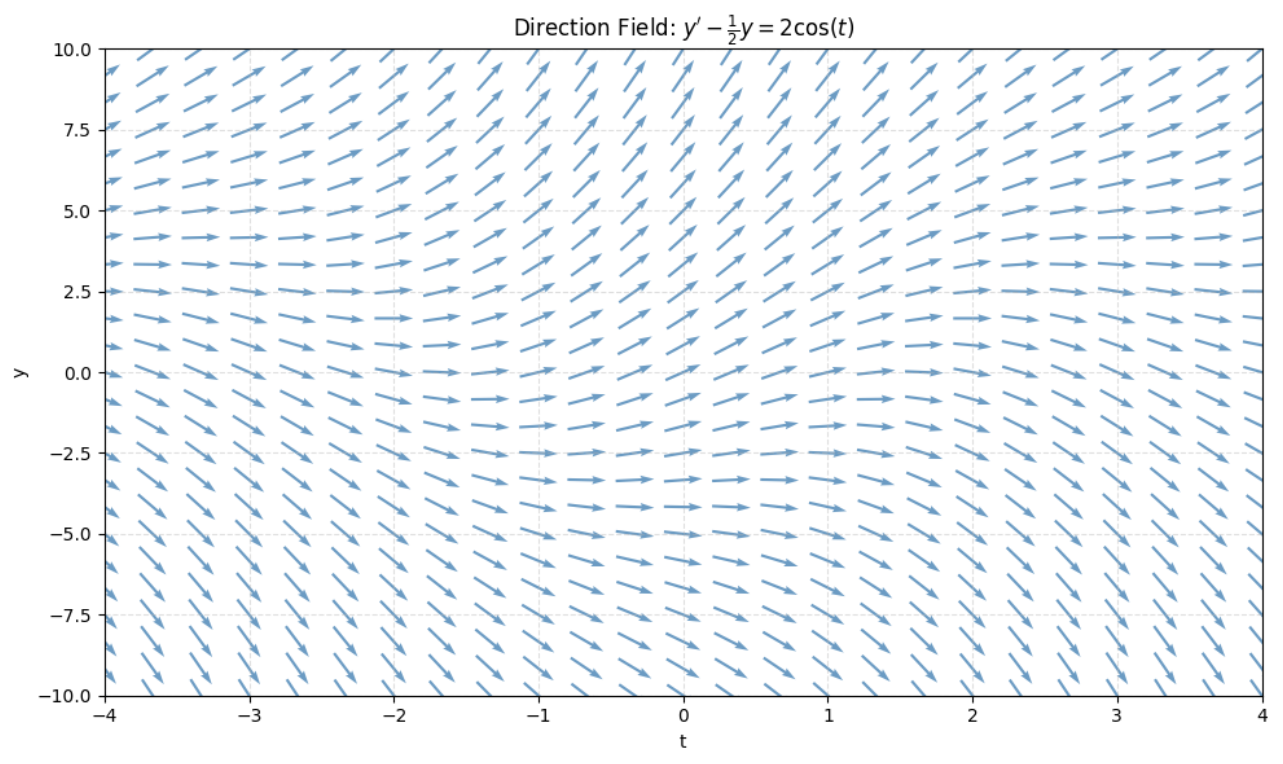
\includegraphics[width=0.8\textwidth]{secciones/michael/images/DF_13.png}
    \caption{Direction field for $y' - \frac{1}{2}y = 2\cos(t)$}
    \label{fig:dirfield}
\end{figure}

The solutions clearly diverge between $-\infty$ and $+\infty$, and the long-term 
behavior depends entirely on the choice of the initial value $a$. Observing the 
direction field, there exists a critical value $a_0$ at which the transition between 
these two types of behavior occurs. For initial values $a > a_0$ the solutions grow 
toward $+\infty$, while for $a < a_0$ they tend toward $-\infty$. From the direction 
field, this critical value can be estimated as $a_0 \approx -1.3$.


\textbf{2. } Solve the initial value problem and find the critical value $a_0$ exactly.

We solve the equation $y' - \frac{1}{2}y = 2\cos(t)$ using the integrating factor method.

The integrating factor is:
\[
\mu(t) = e^{\int -\frac{1}{2}\,dt} = e^{-\frac{t}{2}}
\]

Multiplying both sides by $\mu(t)$:
\[
\frac{d}{dt}\left(e^{-\frac{t}{2}}\,y\right) = 2e^{-\frac{t}{2}}\cos(t)
\]

Integrating the right-hand side using the formula 
$\displaystyle\int e^{at}\cos(bt)\,dt = \frac{e^{at}(a\cos(bt)+b\sin(bt))}{a^2+b^2}$, 
with $a = -\frac{1}{2}$ and $b = 1$:
\[
\int 2e^{-\frac{t}{2}}\cos(t)\,dt 
\]
\[
= 2\cdot\frac{e^{-\frac{t}{2}}\!\left(-\frac{1}{2}\cos(t)+\sin(t)\right)}{\frac{1}{4}+1}+C
\]
\[
= \frac{8}{5}e^{-\frac{t}{2}}\!\left(-\frac{1}{2}\cos(t)+\sin(t)\right)+C
\]


Thus:
\[
e^{-\frac{t}{2}}\,y = \frac{8}{5}e^{-\frac{t}{2}}\!\left(-\frac{1}{2}\cos(t)+\sin(t)\right)+C
\]

Multiplying through by $e^{\frac{t}{2}}$:
\[
y(t) = \frac{8}{5}\left(-\frac{1}{2}\cos(t)+\sin(t)\right) + Ce^{\frac{t}{2}}
= -\frac{4}{5}\cos(t) + \frac{8}{5}\sin(t) + Ce^{\frac{t}{2}}
\]

Applying the initial condition $y(0) = a$:
\[
a = -\frac{4}{5}\cos(0) + \frac{8}{5}\sin(0) + C = -\frac{4}{5} + C
\implies C = a + \frac{4}{5}
\]

So the solution to the IV is:
\[
\boxed{y(t) = -\frac{4}{5}\cos(t) + \frac{8}{5}\sin(t) + \left(a+\frac{4}{5}\right)e^{\frac{t}{2}}}
\]

Since $e^{t/2} \to +\infty$ as $t \to \infty$, the long-term behavior is governed entirely 
by the sign of the coefficient $C = a + \frac{4}{5}$:

\begin{itemize}
    \item If $a > -\dfrac{4}{5}$, then $C > 0$ and $y(t) \to +\infty$.
    \item If $a < -\dfrac{4}{5}$, then $C < 0$ and $y(t) \to -\infty$.
    \item If $a = -\dfrac{4}{5}$, then $C = 0$ and $y(t)$ oscillates boundedly.
\end{itemize}

Therefore, the exact critical value is:
\[
a_0 = -\frac{4}{5}
\]

This confirms and refines the estimate $a_0 \approx -1.3$ from the direction field 
(the true value $-0.8$ lies in the same region).




\textbf{3. } Describe the behavior of the solution corresponding to the initial value $a_0$.

When $a = a_0 = -\dfrac{4}{5}$, the constant $C = 0$, and the solution reduces to:
\[
y(t) = -\frac{4}{5}\cos(t) + \frac{8}{5}\sin(t)
\]

This can be written in amplitude-phase form as $y(t) = R\cos(t - \phi)$, where:
\[
R = \sqrt{\left(\frac{4}{5}\right)^2 + \left(\frac{8}{5}\right)^2} 
= \sqrt{\frac{16+64}{25}} = \sqrt{\frac{80}{25}} = \frac{4\sqrt{5}}{5}
\]

Therefore, when $a = a_0$, the solution is purely oscillatory with amplitude 
$\dfrac{4\sqrt{5}}{5} \approx 1.789$ and period $2\pi$. It neither grows nor decays 
as $t \to \infty$, in contrast to all other solutions which are eventually dominated 
by the $e^{t/2}$ term and diverge to $\pm\infty$.

\end{respuesta}




\begin{center}
    \rule{0.5\textwidth}{0.5pt}
\end{center}



\textbf{14. $3y' - 2y = e^{-\pi t/2}, \quad y(0) = a$}
\begin{respuesta}

\textbf{1. }Draw a direction field for the given differential equation. How do solutions appear to behave as $t$ becomes large? Does the behavior depend on the choice of the initial value $a$? Let $a_0$ be the value of $a$ for which the transition from one type of behavior to another occurs. Estimate the value of $a_0$.
\begin{figure}[H]
    \centering
    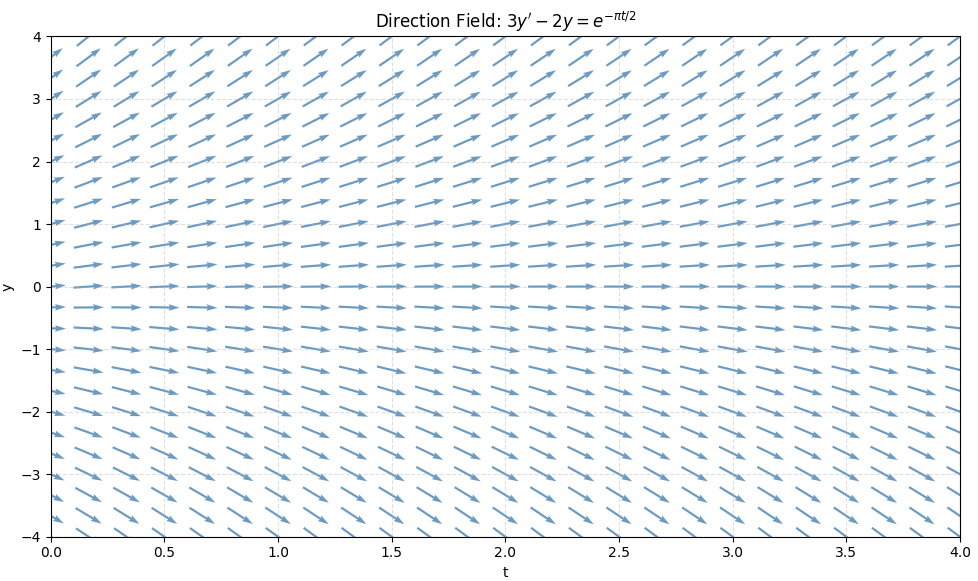
\includegraphics[width=0.8\textwidth]{secciones/michael/images/DF_14.png}
    \caption{Direction field for $3y' - 2y = e^{-\pi t/2}, \quad y(0) = a$}
    \label{fig:dirfield}
\end{figure}

The solutions clearly diverge between $-\infty$ and $+\infty$, and the long-term 
behavior depends entirely on the choice of the initial value $a$. Observing the 
direction field, there exists a critical value $a_0$ at which the transition between 
these two types of behavior occurs. For initial values $a > a_0$ the solutions grow 
toward $+\infty$, while for $a < a_0$ they tend toward $-\infty$. From the direction 
field, this critical value can be estimated as $a_0 \approx 0$. Even when this is an approximation I'm almost completely sure that is the critical value.


\textbf{2. }Solve the initial value problem and find the critical value $a_0$ exactly.

We rewrite the equation in standard form:
\[
y' - \frac{2}{3}y = \frac{1}{3}e^{-\pi t/2}
\]

The integrating factor is:
\[
\mu(t) = e^{\int -\frac{2}{3}\,dt} = e^{-\frac{2}{3}t}
\]

Multiplying both sides by $\mu(t)$:
\[
\frac{d}{dt}\left[e^{-\frac{2}{3}t}\,y\right] = \frac{1}{3}e^{-\frac{2}{3}t}\cdot e^{-\frac{\pi}{2}t} = \frac{1}{3}e^{-\left(\frac{2}{3}+\frac{\pi}{2}\right)t}
\]

Integrating both sides:
\[
e^{-\frac{2}{3}t}\,y = \frac{1}{3} \cdot \frac{1}{-\left(\frac{2}{3}+\frac{\pi}{2}\right)}e^{-\left(\frac{2}{3}+\frac{\pi}{2}\right)t} + C
\]

\[
e^{-\frac{2}{3}t}\,y = \frac{-1}{3\left(\frac{2}{3}+\frac{\pi}{2}\right)}e^{-\left(\frac{2}{3}+\frac{\pi}{2}\right)t} + C
\]

Simplifying the constant. Let $k = \dfrac{2}{3}+\dfrac{\pi}{2} = \dfrac{4+3\pi}{6}$, so:

\[
e^{-\frac{2}{3}t}\,y = \frac{-1}{3k}\,e^{-kt} + C
\]

Multiplying both sides by $e^{\frac{2}{3}t}$:
\[
y = \frac{-1}{3k}\,e^{-\left(k-\frac{2}{3}\right)t} + Ce^{\frac{2}{3}t}
\]

Since $k - \dfrac{2}{3} = \dfrac{\pi}{2}$, we get:
\[
y = \frac{-1}{3k}\,e^{-\frac{\pi}{2}t} + Ce^{\frac{2}{3}t}
\]

Applying the initial condition $y(0) = a$:
\[
a = \frac{-1}{3k} + C \implies C = a + \frac{1}{3k}
\]

So the solution is:
\[
\boxed{y(t) = \frac{-1}{3k}\,e^{-\frac{\pi}{2}t} + \left(a + \frac{1}{3k}\right)e^{\frac{2}{3}t}}, \qquad k = \frac{4+3\pi}{6}
\]

\textbf{Finding the critical value $a_0$:}

As $t \to \infty$, the term $e^{-\frac{\pi}{2}t} \to 0$, so the long-term behavior is governed entirely by the term $\left(a + \dfrac{1}{3k}\right)e^{\frac{2}{3}t}$.

\begin{itemize}
    \item If $a + \dfrac{1}{3k} > 0$, then $y \to +\infty$.
    \item If $a + \dfrac{1}{3k} < 0$, then $y \to -\infty$.
    \item If $a + \dfrac{1}{3k} = 0$, the exponential growth term vanishes and $y \to 0$.
\end{itemize}

Therefore, the exact critical value is:
\[
\boxed{a_0 = -\frac{1}{3k} = -\frac{2}{4+3\pi} \approx -0.132}
\]

This confirms our earlier estimate: $a_0$ is close to $0$, but the exact value is $a_0 = -\dfrac{2}{4+3\pi}$.



\textbf{3. }Describe the behavior of the solution corresponding to the initial value $a_0$.

For the critical initial value $a_0 = -\dfrac{2}{4+3\pi}$, the coefficient of the 
growing exponential vanishes, i.e., $a_0 + \dfrac{1}{3k} = 0$. The solution reduces to:
\[
y(t) = \frac{-1}{3k}\,e^{-\frac{\pi}{2}t}
\]
Since $-\dfrac{1}{3k} < 0$ and the exponential $e^{-\frac{\pi}{2}t} \to 0$ as 
$t \to \infty$, this solution decays monotonically to zero from below. That is:
\[
\lim_{t \to \infty} y(t) = 0
\]
This is the unique solution that neither grows to $+\infty$ nor diverges to $-\infty$. 
It represents the boundary between the two divergent behaviors.



\end{respuesta}


\noindent In each of Problems 15 and 16:
\begin{enumerate}
    \item Draw a direction field for the given differential equation. How do solutions appear to behave as $t \to 0$? Does the behavior depend on the choice of the initial value $a$? Let $a_0$ be the critical value of $a$, that is, the initial value such that the solutions for $a < a_0$ and the solutions for $a > a_0$ have different behaviors as $t \to \infty$. Estimate the value of $a_0$.
    \item Solve the initial value problem and find the critical value $a_0$ exactly.
    \item Describe the behavior of the solution corresponding to the initial value $a_0$.
\end{enumerate}


\begin{center}
    \rule{0.5\textwidth}{0.5pt}
\end{center}



\textbf{16. $(\sin(t))y' + (\cos(t))y = e^t, \quad y(1) = a, \quad 0 < t < \pi$}
\begin{respuesta}

\textbf{1. }Draw a direction field for the given differential equation. How do solutions appear to behave as $t \to 0$? Does the behavior depend on the choice of the initial value $a$? Let $a_0$ be the critical value of $a$, that is, the initial value such that the solutions for $a < a_0$ and the solutions for $a > a_0$ have different behaviors as $t \to \infty$. Estimate the value of $a_0$.

\begin{figure}[H]
    \centering
    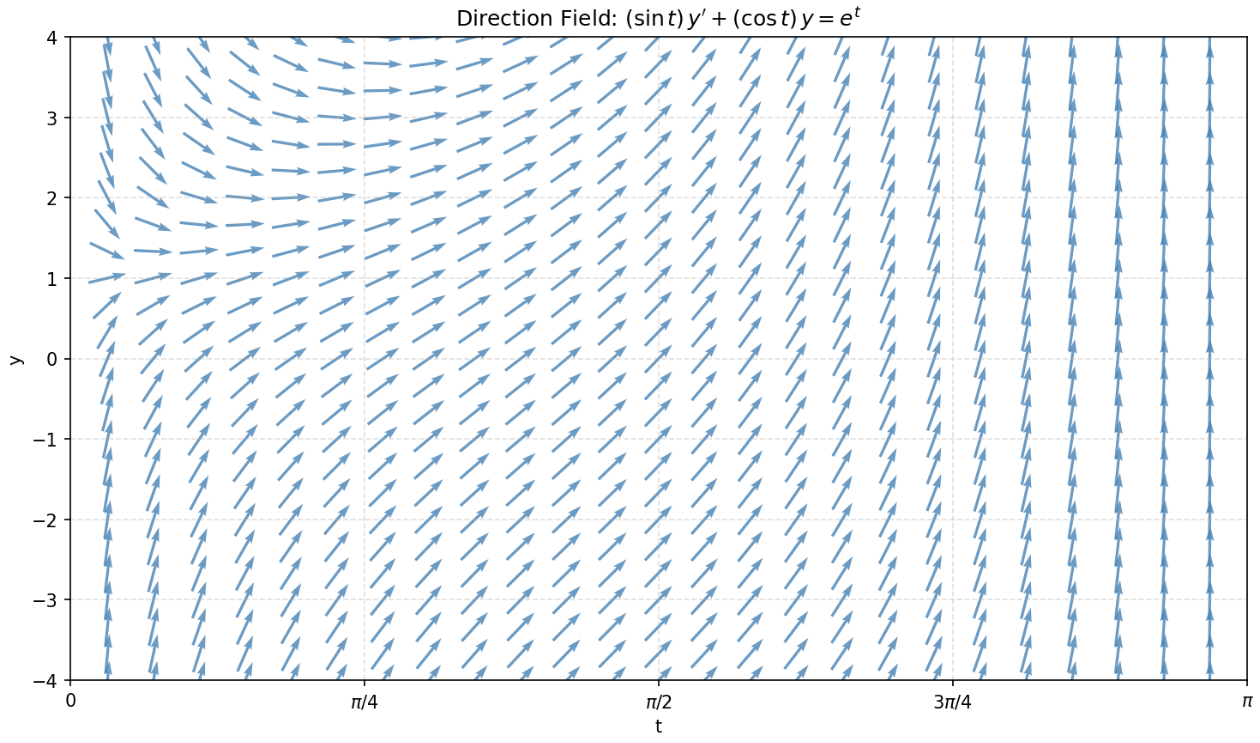
\includegraphics[width=0.8\textwidth]{secciones/michael/images/DF_16.png}
    \caption{Direction field for $(\sin(t))y' + (\cos(t))y = e^t, \quad y(1) = a, \quad 0 < t < \pi$}
    \label{fig:dirfield}
\end{figure}

From the direction field, as $t \to 0^+$ the slopes become increasingly 
steep, suggesting that solutions grow without bound near the left endpoint regardless 
of the initial value $a$; that is, this singular behavior does not depend on the 
choice of $a$. The D.F doesn't show any critical value in the long therm solutions of the possible functions, in that order of ideas when $t$ tends to $\infty$ the solutions is as well up without any bound.

\textbf{2. }Solve the initial value problem and find the critical value $a_0$ exactly.

The left-hand side is an exact derivative:
\[
(\sin t)\,y' + (\cos t)\,y = \frac{d}{dt}\bigl[\sin(t)\cdot y\bigr]
\]
so the equation becomes:
\[
\frac{d}{dt}\bigl[\sin(t)\cdot y\bigr] = e^t
\]
Integrating both sides directly:
\[
\sin(t)\cdot y = e^t + C
\]
\[
y = \frac{e^t + C}{\sin t}
\]
Applying the initial condition $y(1) = a$:
\[
a = \frac{e^1 + C}{\sin 1} \implies C = a\sin(1) - e
\]
So the solution to the initial value problem is:
\[
\boxed{y(t) = \frac{e^t + a\sin(1) - e}{\sin t}}
\]

\textbf{Finding the critical value $a_0$:} As $t \to \pi^-$, we have $\sin t \to 0^+$, 
so the behavior of $y(t)$ is governed entirely by the sign of the numerator 
$e^t + a\sin(1) - e$ evaluated at $t = \pi$:
\begin{itemize}
    \item If $e^\pi + a\sin(1) - e > 0$, then $y \to +\infty$.
    \item If $e^\pi + a\sin(1) - e < 0$, then $y \to -\infty$.
    \item If $e^\pi + a\sin(1) - e = 0$, the numerator vanishes and the transition occurs.
\end{itemize}
Setting the numerator equal to zero:
\[
e^\pi + a_0\sin(1) - e = 0 \implies a_0 = \frac{e - e^\pi}{\sin(1)}
\]
\[
\boxed{a_0 = \frac{e - e^\pi}{\sin(1)} \approx -0.172}
\]



\textbf{3. }Describe the behavior of the solution corresponding to the initial value $a_0$.

For the critical initial value $a_0 = \dfrac{e - e^\pi}{\sin(1)}$, 
the numerator of the solution vanishes as $t \to \pi^-$, so the growing exponential 
term is exactly cancelled. The solution reduces to:
\[
y(t) = \frac{e^t - e^\pi}{\sin t}
\]
which remains bounded and decreases toward zero as $t \to \pi^-$, since both 
numerator and denominator vanish at $t = \pi$. This solution represents the unique 
boundary case that neither diverges to $+\infty$ nor to $-\infty$, separating the 
two divergent behaviors observed for all other initial values.

\end{respuesta}







    
\end{quote}